\documentclass[12pt,a4paper]{report}
\usepackage[utf8]{inputenc}
\usepackage[T1]{fontenc}
\usepackage[english]{babel}
\usepackage{longtable}
\usepackage{booktabs}
\usepackage{graphicx}
\usepackage{float}
\usepackage{tikz}
\usetikzlibrary{arrows.meta,positioning,fit,calc,shapes.geometric}
\usepackage[margin=2.5cm]{geometry}
\usepackage{hyperref}
\begin{document}
\tableofcontents
% =====================================================================
% Chapter 3 -- Requirements Analysis and Specification (Part 1: 3.1 - 3.4)
% Author: Ilyes
%
% Packages required in the main preamble (add only the missing ones):
%   \usepackage{booktabs}
%   \usepackage{array}
%
% Usage in main.tex:  \input{chapter3_part1}   (or paste directly)
% =====================================================================

\chapter{Requirements Analysis and Specification}
\label{chap:requirements}

% ---------------------------------------------------------------------
\section{Introduction}
\label{sec:req-intro}

This chapter sets out what MindSpark must do and how well it must do it. It identifies the actors, lists the functional and non-functional requirements, then presents the global use case diagram, the software architecture and the Scrum backlog that drives the three sprints.



% ---------------------------------------------------------------------
\section{Identification of Actors}
\label{sec:actors}

MindSpark has four actors: three human and one software. Each is described below.

\subsection{Visitor}

The Visitor is a person who is not logged in yet. A visitor can register, log in and ask to reset a forgotten password.

\subsection{Room Creator}

The Room Creator organises a brainstorming session, usually an organizer or facilitator. This actor is also a participant, with extra rights over the rooms he or she creates: sharing the invitation code, editing, closing or deleting the room, removing participants, launching vote pools and exporting results.

\subsection{Participant}

The Participant is any logged-in user who joins a room with an invitation code. Participants add, edit and delete their own ideas, comment, vote, and use the AI assistant within the limits of their plan. They see other people's activity live.

\subsection{AI System (LLM Service)}

The AI System is a backend service that wraps external language models. It generates, expands, groups, summarises and compares ideas, detects risks, and builds action plans, within each user's daily quota.

\subsection{Mapping Between Backlog Roles and Actors}

The backlog stories use roles such as visitor, user, client or developer. Table~\ref{tab:role-mapping} maps them to the three actors. ``Client'' means any logged-in user, so it covers both the Participant and the Room Creator. Developer and team stories are technical enablers, covered in Section~3.7.

\begin{table}[htbp]
\centering
\caption{Mapping between backlog roles and actors}
\label{tab:role-mapping}
\begin{tabular}{@{}p{0.30\textwidth}p{0.60\textwidth}@{}}
\toprule
\textbf{Role in the backlog} & \textbf{Actor} \\
\midrule
Visitor & Visitor \\
User, Client & Participant (and Room Creator, who inherits all participant rights) \\
Room creator & Room Creator \\
Developer & Technical stories for the development team (T1 to T7) \\
\bottomrule
\end{tabular}
\end{table}

% ---------------------------------------------------------------------
\section{Functional Requirements Specification}
\label{sec:functional}

The functional requirements come from the backlog stories and are grouped into six families. The story IDs in brackets link each requirement to its user story. Priorities and sprints are given in the product backlog (Section~3.7). Story numbers follow the original user-story document, so some are skipped, such as US-31.

\subsection{Account and Profile Management}
\label{subsec:fr-account}

Registration, login, profile and password. Credentials are handled by a separate identity provider, not by the business services.

\noindent The system shall:
\begin{itemize}
  \item allow a visitor to register with a name, an email address and a password (US-1)
  \item allow a user to log in and log out (US-2, US-3)
  \item let a user view his or her profile and edit his or her name and avatar (US-4, US-5)
  \item let a user reset a forgotten password by email and change his or her password (US-6, US-7)
  \item let a user delete his or her account (US-8)
\end{itemize}

\subsection{Brainstorming Room Management}
\label{subsec:fr-rooms}

A room is the shared space where a session happens. These requirements cover its whole life, from creation to deletion.

\noindent The system shall:
\begin{itemize}
  \item allow a user to create a brainstorming room (US-9)
  \item allow a user to join a room with an invitation code and to leave it (US-10, US-11)
  \item list the rooms a user created and let him or her reopen them later (US-12)
  \item allow the room creator to edit the room details (US-13)
  \item allow the room creator to preview the participants and remove one (US-14, US-15)
  \item allow the room creator to close or delete the room (US-16, US-17)
\end{itemize}

\subsection{Ideas, Media, Categories, Comments and Voting}
\label{subsec:fr-ideas}

The core of the platform: creating and organising ideas, discussing them and voting.

\noindent The system shall:
\begin{itemize}
  \item allow a user to create, edit and delete his or her own ideas in a room he or she belongs to (US-22 to US-24)
  \item display all the ideas of the room to its participants (US-25)
  \item allow a user to attach images to an idea (US-26)
  \item allow a user to organise ideas into categories and to create, rename and delete categories (US-27, US-28)
  \item allow a user to search ideas by keyword, and to filter them by category, author and minimum votes and sort them (US-29, US-30)
  \item allow a user to comment on an idea, edit or delete his or her comments, and reply to a comment (US-32 to US-34)
  \item allow a user to vote for an idea and to remove or change his or her vote (US-35, US-36)
  \item allow the room creator to create a vote pool (US-37)
\end{itemize}

\subsection{Real-Time Collaboration}
\label{subsec:fr-realtime}

What one participant does appears for everyone else without reloading the page.

\noindent The system shall:
\begin{itemize}
  \item provide an authenticated real-time channel for each room (technical enabler) (US-38)
  \item show new ideas, comments and votes to all participants live (US-39)
  \item show which participants are online in the room (US-40)
  \item show the cursors of the other participants live (US-41)
\end{itemize}

\subsection{AI Ideation and Analytical Assistant}
\label{subsec:fr-ai}

AI helps in two ways: producing and improving ideas, then grouping, evaluating and summarising them.

\noindent The system shall:
\begin{itemize}
  \item provide a backend AI service that wraps the LLM provider (technical enabler) (US-42)
  \item generate ideas with AI from a topic (US-43)
  \item improve or expand an idea with AI (US-44)
  \item group similar ideas with AI (US-45)
  \item summarise a brainstorming session with AI (US-46)
  \item find risks in a selected idea with AI (US-47)
  \item compare two to four selected ideas with AI (US-48)
  \item convert selected ideas into an action plan (US-49)
\end{itemize}

\subsection{History, Export and Subscriptions}
\label{subsec:fr-history}

Saving and exporting sessions, and the subscription model.

\noindent The system shall:
\begin{itemize}
  \item let a user save and revisit his or her brainstorming sessions (US-52)
  \item let a user export the results of a session (US-53)
  \item show the available plans and let a user subscribe to one (US-54, US-55)
  \item let a user upgrade, downgrade or cancel his or her plan (US-56, US-57)
  \item let a user view his or her billing history (US-58)
  \item keep each user within the limits of his or her plan (rooms, participants, AI calls) and refuse requests beyond them (US-59)
\end{itemize}

% ---------------------------------------------------------------------
\section{Non-Functional Requirements Specification}
\label{sec:nonfunctional}

These requirements describe the quality the platform must reach, beyond its features.

\paragraph{NFR-1: Low-latency real-time synchronisation.}
Changes and presence information must reach the other participants almost instantly. High-frequency messages such as cursor moves are rate-limited, and updates are sent only after the database transaction commits.

\paragraph{NFR-2: Channel isolation and authenticated room channels.}
Each room has its own channel. A connection needs a valid token and room membership, and events never reach users outside the room.

\paragraph{NFR-3: Authentication and role-based security.}
Users log in through a central identity provider that issues JWTs, which each service checks locally. Roles control access. Internal endpoints are not exposed publicly, and secrets stay out of logs and code.

\paragraph{NFR-4: API quota enforcement.}
The server enforces plan limits on active rooms, participants per room and daily AI calls, and returns a clear error when a limit is reached. The AI service also caps simultaneous calls to the providers.

\paragraph{NFR-5: Responsiveness and usability.}
The interface must work on laptops and tablets, stay fluid when dragging ideas, and show feedback during slow AI requests.

\paragraph{NFR-6: Reliability and fault tolerance.}
One failing service must not take down the platform. Calls use timeouts and circuit breakers, the AI service can switch provider, and model output is validated before it is displayed.

\paragraph{NFR-7: Data integrity and concurrency.}
Simultaneous actions on the same object, such as two users dragging one card, must not corrupt data. Short soft locks handle this, and deleted items must not reappear.

\paragraph{NFR-8: Automated testing (T6).}
Critical flows must be covered by automated tests that pass before release. Results are in Chapter~6.

\paragraph{NFR-9: Platform hardening (T7).}
Before real users arrive: lock down management endpoints, validate uploaded files by content, limit service memory, and check that no secret leaks. Results are in Chapter~6.

\paragraph{NFR-10: Maintainability, observability and deployability.}
The platform must be modular, centrally configured and containerised, so the whole environment starts with one command. Metrics and traces help diagnose problems.


Table~\ref{tab:nfr-summary} summarises these requirements and where they are addressed.

\begin{table}[htbp]
\centering
\caption{Summary of non-functional requirements}
\label{tab:nfr-summary}
\begin{tabular}{@{}p{0.09\textwidth}p{0.42\textwidth}p{0.18\textwidth}p{0.14\textwidth}@{}}
\toprule
\textbf{ID} & \textbf{Quality attribute} & \textbf{Related stories} & \textbf{Main sprint} \\
\midrule
NFR-1 & Low-latency real-time synchronisation & US-38 to US-41 & Sprint 2 \\
NFR-2 & Channel isolation, authenticated channels & US-38, US-10, US-15 & Sprint 2 \\
NFR-3 & Authentication and role-based security & US-1, US-2, US-3 & Sprints 1 and 3 \\
NFR-4 & Quota enforcement & US-42 to US-44, US-59 & Sprints 2 and 3 \\
NFR-5 & Responsiveness and usability & All client stories & Sprints 1 to 3 \\
NFR-6 & Reliability and fault tolerance & US-42, US-45 to US-49 & Sprints 2 and 3 \\
NFR-7 & Data integrity and concurrency & US-22 to US-24, US-39 & Sprints 1 and 2 \\
NFR-8 & Automated testing & T6 & Sprint 3 \\
NFR-9 & Platform hardening & T7 & Sprint 3 \\
NFR-10 & Maintainability, observability, deployability & T1 to T4 & Sprint 1 \\
\bottomrule
\end{tabular}
\end{table}

% =====================================================================
% Chapter 3 -- Part 3: Section 3.5 (General Use Case Diagram)
% Author: Ilyes
%
% All diagrams are pure TikZ (no image files). Needs in the preamble:
%   \usepackage{tikz}
%   \usetikzlibrary{arrows.meta,positioning,fit,calc,shapes.geometric}
%   \usepackage{graphicx}
%   \usepackage{float}   % keeps each figure under its title (each diagram gets its own page)
% =====================================================================

% \umlactor{name}{x}{y}{label}{dx}: stick figure at (x,y). Creates the
% coordinates (name), (name-top) and (name-bot) used by the arrows.
\providecommand{\umlactor}[5]{%
  \begin{scope}[shift={(#2,#3)}]
    \draw (0,0.5) circle (0.15);
    \draw (0,0.35) -- (0,-0.1);
    \draw (-0.25,0.22) -- (0.25,0.22);
    \draw (0,-0.1) -- (-0.2,-0.5);
    \draw (0,-0.1) -- (0.2,-0.5);
    \node[font=\scriptsize\bfseries, align=center, text width=1.9cm, below] at (0,-0.5) {#4};
  \end{scope}
  \coordinate (#1) at ($(#2,#3)+(#5,0.1)$);
  \coordinate (#1-top) at ($(#2,#3)+(0,0.72)$);
  \coordinate (#1-bot) at ($(#2,#3)+(0,-1.1)$);
}
\providecommand{\fitwidth}[1]{\resizebox{\ifdim\width>\linewidth\linewidth\else\width\fi}{!}{#1}}

% ---------------------------------------------------------------------
\section{General Use Case Diagram}
\label{sec:usecase}

MindSpark has around 70 use cases shared between several actors. Drawing all of them in one figure would make it too crowded to read, so the general use case diagram is split into an overview and nine thematic diagrams. In the thematic diagrams, dashed arrows show include and extend relations, and the grey ovals are shared steps such as \textit{Authenticate} and \textit{Enter room}.

\clearpage
\subsection{Overview}
\label{subsec:uc-overview}

The overview shows who uses MindSpark and which main areas it covers. The Visitor can only register and log in. The Participant uses every other area: account and notifications, rooms, ideas, real-time collaboration, drawing, voting, the AI assistant, saved sessions and the subscription. The Room Creator is a Participant who can also run vote pools, and who has extra moderation rights over rooms and categories, shown in the thematic diagrams. The AI System serves the requests of the AI assistant.

\begin{figure}[H]
\centering
\hyphenpenalty=10000\relax
\fitwidth{%
\begin{tikzpicture}[uc/.style={ellipse, draw, align=center, font=\scriptsize, minimum width=4.2cm, minimum height=0.85cm, text width=3.1cm, inner sep=1pt, fill=white}, sup/.style={uc, fill=gray!12, minimum width=2.8cm, text width=2.0cm}, rel/.style={-{Stealth[length=1.8mm]}, dashed, thin}, lab/.style={font=\tiny, fill=white, inner sep=0.5pt}]
\draw[rounded corners=3pt, thick] (3.40,-11.90) rectangle (8.60,1.35);
\node[font=\small\bfseries, anchor=north west] at (3.50,1.30) {MindSpark};
\node[uc] (G0) at (6.00,0.00) {Register and log in};
\node[uc] (G1) at (6.00,-1.10) {Manage account and notifications};
\node[uc] (G2) at (6.00,-2.20) {Manage rooms};
\node[uc] (G3) at (6.00,-3.30) {Manage ideas and categories};
\node[uc] (G4) at (6.00,-4.40) {Collaborate in real time};
\node[uc] (G5) at (6.00,-5.50) {Draw on the canvas};
\node[uc] (G6) at (6.00,-6.60) {Vote on ideas};
\node[uc] (G7) at (6.00,-7.70) {Use AI assistant};
\node[uc] (G8) at (6.00,-8.80) {Save and export sessions};
\node[uc] (G9) at (6.00,-9.90) {Manage subscription};
\node[uc] (G10) at (6.00,-11.00) {Vote pool};
\umlactor{V}{0.90}{0.00}{Visitor}{0.3}
\umlactor{P}{0.90}{-5.50}{Participant}{0.3}
\umlactor{C}{0.90}{-11.00}{Room Creator}{0.3}
\draw (V) -- (G0.west);
\draw (P) -- (G1.west);
\draw (P) -- (G2.west);
\draw (P) -- (G3.west);
\draw (P) -- (G4.west);
\draw (P) -- (G5.west);
\draw (P) -- (G6.west);
\draw (P) -- (G7.west);
\draw (P) -- (G8.west);
\draw (P) -- (G9.west);
\draw (C) -- (G10.west);
\draw[-{Triangle[open,length=2.6mm,width=2.6mm]}, thick] (C-top) -- (P-bot);
\end{tikzpicture}}
\caption{General use case diagram: overview}
\label{fig:uc-overview}
\end{figure}

\clearpage
\subsection{Account and Notifications}
\label{subsec:uc-account}

This diagram covers registration, login, password reset, account deletion and notifications.

\begin{figure}[H]
\centering
\hyphenpenalty=10000\relax
\fitwidth{%
\begin{tikzpicture}[uc/.style={ellipse, draw, align=center, font=\scriptsize, minimum width=4.2cm, minimum height=0.85cm, text width=3.1cm, inner sep=1pt, fill=white}, sup/.style={uc, fill=gray!12, minimum width=2.8cm, text width=2.0cm}, rel/.style={-{Stealth[length=1.8mm]}, dashed, thin}, lab/.style={font=\tiny, fill=white, inner sep=0.5pt}]
\draw[rounded corners=3pt, thick] (3.40,-10.80) rectangle (12.90,1.35);
\node[font=\small\bfseries, anchor=north west] at (3.50,1.30) {MindSpark};
\node[uc] (C1) at (6.00,0.00) {Register};
\node[uc] (C2) at (6.00,-1.10) {Log in};
\node[uc] (C3) at (6.00,-2.20) {Forgot password};
\node[uc] (C4) at (6.00,-3.30) {Send reset code by email};
\node[uc] (C5) at (6.00,-4.40) {Reset password};
\node[uc] (C6) at (6.00,-5.50) {Log out};
\node[uc] (C7) at (6.00,-6.60) {Delete account};
\node[uc] (C8) at (6.00,-7.70) {View notifications};
\node[uc] (C9) at (6.00,-8.80) {Mark notification as read};
\node[uc] (C10) at (6.00,-9.90) {Delete notification};
\node[sup] (AUTH) at (11.00,-7.15) {Authenticate};
\umlactor{V}{0.90}{-1.10}{Visitor}{0.3}
\umlactor{P}{0.90}{-7.15}{Participant}{0.3}
\draw (V) -- (C1.west);
\draw (V) -- (C2.west);
\draw (V) -- (C3.west);
\draw (P) -- (C5.west);
\draw (P) -- (C6.west);
\draw (P) -- (C7.west);
\draw (P) -- (C8.west);
\draw (P) -- (C9.west);
\draw (P) -- (C10.west);
\draw[rel] (C3.east) to[out=0,in=0,looseness=1.6] node[lab,pos=0.45]{\guillemotleft include\guillemotright} (C4.east);
\draw[rel] (C3.east) to[out=0,in=0,looseness=1.6] node[lab,pos=0.45]{\guillemotleft include\guillemotright} (C5.east);
\draw[rel] (C5.east) -- node[lab,pos=0.45]{\guillemotleft include\guillemotright} (AUTH.west);
\draw[rel] (C6.east) --  (AUTH.west);
\draw[rel] (C7.east) --  (AUTH.west);
\draw[rel] (C8.east) --  (AUTH.west);
\draw[rel] (C9.east) --  (AUTH.west);
\draw[rel] (C10.east) --  (AUTH.west);
\end{tikzpicture}}
\caption{Use case diagram: account and notifications}
\label{fig:uc-account}
\end{figure}

\clearpage
\subsection{Room Management}
\label{subsec:uc-rooms}

This diagram covers creating, joining, leaving and moderating rooms.

\begin{figure}[H]
\centering
\hyphenpenalty=10000\relax
\fitwidth{%
\begin{tikzpicture}[uc/.style={ellipse, draw, align=center, font=\scriptsize, minimum width=4.2cm, minimum height=0.85cm, text width=3.1cm, inner sep=1pt, fill=white}, sup/.style={uc, fill=gray!12, minimum width=2.8cm, text width=2.0cm}, rel/.style={-{Stealth[length=1.8mm]}, dashed, thin}, lab/.style={font=\tiny, fill=white, inner sep=0.5pt}]
\draw[rounded corners=3pt, thick] (3.40,-9.70) rectangle (16.50,1.35);
\node[font=\small\bfseries, anchor=north west] at (3.50,1.30) {MindSpark};
\node[uc] (A1) at (6.00,0.00) {Create room};
\node[uc] (A2) at (6.00,-1.10) {Join room with invitation code};
\node[uc] (A4) at (6.00,-2.20) {Leave room};
\node[uc] (A3) at (6.00,-3.30) {View my rooms};
\node[uc] (B1) at (6.00,-4.40) {Rename room};
\node[uc] (B2) at (6.00,-5.50) {Remove participant};
\node[uc] (B3) at (6.00,-6.60) {Close room};
\node[uc] (B4) at (6.00,-7.70) {Reopen room};
\node[uc] (B5) at (6.00,-8.80) {Delete room};
\node[sup] (ENTER) at (11.00,-3.30) {Enter room};
\node[sup] (AUTH) at (14.60,-5.78) {Authenticate};
\umlactor{P}{0.90}{-1.98}{Participant}{0.3}
\umlactor{C}{0.90}{-6.60}{Room Creator}{0.3}
\draw (P) -- (A1.west);
\draw (P) -- (A2.west);
\draw (P) -- (A4.west);
\draw (P) -- (A3.west);
\draw (P) -- (ENTER.west);
\draw (C) -- (B1.west);
\draw (C) -- (B2.west);
\draw (C) -- (B3.west);
\draw (C) -- (B4.west);
\draw (C) -- (B5.west);
\draw[rel] (A1.east) -- node[lab,pos=0.45]{\guillemotleft include\guillemotright} (ENTER.west);
\draw[rel] (A2.east) --  (ENTER.west);
\draw[rel] (A4.east) --  (ENTER.west);
\draw[rel] (B1.east) --  (ENTER.west);
\draw[rel] (B2.east) --  (ENTER.west);
\draw[rel] (B3.east) --  (ENTER.west);
\draw[rel] (ENTER.east) -- node[lab,pos=0.45]{\guillemotleft include\guillemotright} (AUTH.west);
\draw[rel] (A3.east) --  (AUTH.west);
\draw[rel] (B4.east) --  (AUTH.west);
\draw[rel] (B5.east) --  (AUTH.west);
\draw[-{Triangle[open,length=2.6mm,width=2.6mm]}, thick] (C-top) -- (P-bot);
\end{tikzpicture}}
\caption{Use case diagram: room management}
\label{fig:uc-rooms}
\end{figure}

\clearpage
\subsection{Ideas and Organisation}
\label{subsec:uc-ideas}

This diagram covers ideas, images, categories, search, filters and sorting.

\begin{figure}[H]
\centering
\hyphenpenalty=10000\relax
\fitwidth{%
\begin{tikzpicture}[uc/.style={ellipse, draw, align=center, font=\scriptsize, minimum width=4.2cm, minimum height=0.85cm, text width=3.1cm, inner sep=1pt, fill=white}, sup/.style={uc, fill=gray!12, minimum width=2.8cm, text width=2.0cm}, rel/.style={-{Stealth[length=1.8mm]}, dashed, thin}, lab/.style={font=\tiny, fill=white, inner sep=0.5pt}]
\draw[rounded corners=3pt, thick] (3.40,-10.80) rectangle (16.50,1.35);
\node[font=\small\bfseries, anchor=north west] at (3.50,1.30) {MindSpark};
\node[uc] (C1) at (6.00,0.00) {Create idea};
\node[uc] (C2) at (6.00,-1.10) {Edit own idea};
\node[uc] (C3) at (6.00,-2.20) {Delete own idea};
\node[uc] (C4) at (6.00,-3.30) {View ideas};
\node[uc] (C5) at (6.00,-4.40) {Attach images to idea};
\node[uc] (C6) at (6.00,-5.50) {Assign idea to category};
\node[uc] (C7) at (6.00,-6.60) {Search ideas};
\node[uc] (C8) at (6.00,-7.70) {Filter by category};
\node[uc] (C9) at (6.00,-8.80) {Sort ideas};
\node[uc] (C10) at (6.00,-9.90) {Manage categories};
\node[sup] (ENTER) at (11.00,-4.95) {Enter room};
\node[sup] (AUTH) at (14.60,-4.95) {Authenticate};
\umlactor{P}{0.90}{-4.40}{Participant}{0.3}
\umlactor{C}{0.90}{-9.90}{Room Creator}{0.3}
\draw (P) -- (C1.west);
\draw (P) -- (C2.west);
\draw (P) -- (C3.west);
\draw (P) -- (C4.west);
\draw (P) -- (C5.west);
\draw (P) -- (C6.west);
\draw (P) -- (C7.west);
\draw (P) -- (C8.west);
\draw (P) -- (C9.west);
\draw (C) -- (C10.west);
\draw[rel] (C1.east) -- node[lab,pos=0.45]{\guillemotleft include\guillemotright} (ENTER.west);
\draw[rel] (C2.east) --  (ENTER.west);
\draw[rel] (C3.east) --  (ENTER.west);
\draw[rel] (C4.east) --  (ENTER.west);
\draw[rel] (C5.east) --  (ENTER.west);
\draw[rel] (C6.east) --  (ENTER.west);
\draw[rel] (C7.east) --  (ENTER.west);
\draw[rel] (C8.east) --  (ENTER.west);
\draw[rel] (C9.east) --  (ENTER.west);
\draw[rel] (C10.east) --  (ENTER.west);
\draw[rel] (ENTER.east) -- node[lab,pos=0.45]{\guillemotleft include\guillemotright} (AUTH.west);
\draw[-{Triangle[open,length=2.6mm,width=2.6mm]}, thick] (C-top) -- (P-bot);
\end{tikzpicture}}
\caption{Use case diagram: ideas and organisation}
\label{fig:uc-ideas}
\end{figure}

\clearpage
\subsection{Real-Time Collaboration and Comments}
\label{subsec:uc-realtime}

This diagram covers live updates, presence, cursors and comments.

\begin{figure}[H]
\centering
\hyphenpenalty=10000\relax
\fitwidth{%
\begin{tikzpicture}[uc/.style={ellipse, draw, align=center, font=\scriptsize, minimum width=4.2cm, minimum height=0.85cm, text width=3.1cm, inner sep=1pt, fill=white}, sup/.style={uc, fill=gray!12, minimum width=2.8cm, text width=2.0cm}, rel/.style={-{Stealth[length=1.8mm]}, dashed, thin}, lab/.style={font=\tiny, fill=white, inner sep=0.5pt}]
\draw[rounded corners=3pt, thick] (3.40,-6.40) rectangle (16.50,1.35);
\node[font=\small\bfseries, anchor=north west] at (3.50,1.30) {MindSpark};
\node[uc] (C1) at (6.00,0.00) {See live updates};
\node[uc] (C2) at (6.00,-1.10) {See online participants};
\node[uc] (C3) at (6.00,-2.20) {See live cursors};
\node[uc] (C4) at (6.00,-3.30) {Comment on idea};
\node[uc] (C5) at (6.00,-4.40) {Reply to comment};
\node[uc] (C6) at (6.00,-5.50) {Edit or delete own comment};
\node[sup] (ENTER) at (11.00,-2.75) {Enter room};
\node[sup] (AUTH) at (14.60,-2.75) {Authenticate};
\umlactor{P}{0.90}{-2.75}{Participant}{0.3}
\draw (P) -- (C1.west);
\draw (P) -- (C2.west);
\draw (P) -- (C3.west);
\draw (P) -- (C4.west);
\draw (P) -- (C5.west);
\draw (P) -- (C6.west);
\draw[rel] (C1.east) -- node[lab,pos=0.45]{\guillemotleft include\guillemotright} (ENTER.west);
\draw[rel] (C2.east) --  (ENTER.west);
\draw[rel] (C3.east) --  (ENTER.west);
\draw[rel] (C4.east) --  (ENTER.west);
\draw[rel] (C5.east) --  (ENTER.west);
\draw[rel] (C6.east) --  (ENTER.west);
\draw[rel] (ENTER.east) -- node[lab,pos=0.45]{\guillemotleft include\guillemotright} (AUTH.west);
\end{tikzpicture}}
\caption{Use case diagram: real-time collaboration and comments}
\label{fig:uc-realtime}
\end{figure}

\clearpage
\subsection{Drawing and Tools}
\label{subsec:uc-drawing}

This diagram covers the canvas tools: pen, highlighter, shapes, eraser, images and undo.

\begin{figure}[H]
\centering
\hyphenpenalty=10000\relax
\fitwidth{%
\begin{tikzpicture}[uc/.style={ellipse, draw, align=center, font=\scriptsize, minimum width=4.2cm, minimum height=0.85cm, text width=3.1cm, inner sep=1pt, fill=white}, sup/.style={uc, fill=gray!12, minimum width=2.8cm, text width=2.0cm}, rel/.style={-{Stealth[length=1.8mm]}, dashed, thin}, lab/.style={font=\tiny, fill=white, inner sep=0.5pt}]
\draw[rounded corners=3pt, thick] (3.40,-8.60) rectangle (16.50,1.35);
\node[font=\small\bfseries, anchor=north west] at (3.50,1.30) {MindSpark};
\node[uc] (C1) at (6.00,0.00) {Select and move objects};
\node[uc] (C2) at (6.00,-1.10) {Draw with pen};
\node[uc] (C3) at (6.00,-2.20) {Highlight with highlighter};
\node[uc] (C4) at (6.00,-3.30) {Add shapes (circle, triangle, rectangle)};
\node[uc] (C5) at (6.00,-4.40) {Add idea card};
\node[uc] (C6) at (6.00,-5.50) {Erase with eraser};
\node[uc] (C7) at (6.00,-6.60) {Undo and redo};
\node[uc] (C8) at (6.00,-7.70) {Add image to canvas};
\node[sup] (ENTER) at (11.00,-3.85) {Enter room};
\node[sup] (AUTH) at (14.60,-3.85) {Authenticate};
\node[sup] (COL) at (14.60,-2.20) {Choose colour};
\umlactor{P}{0.90}{-3.85}{Participant}{0.3}
\draw (P) -- (C1.west);
\draw (P) -- (C2.west);
\draw (P) -- (C3.west);
\draw (P) -- (C4.west);
\draw (P) -- (C5.west);
\draw (P) -- (C6.west);
\draw (P) -- (C7.west);
\draw (P) -- (C8.west);
\draw[rel] (C1.east) -- node[lab,pos=0.45]{\guillemotleft include\guillemotright} (ENTER.west);
\draw[rel] (C2.east) --  (ENTER.west);
\draw[rel] (C3.east) --  (ENTER.west);
\draw[rel] (C4.east) --  (ENTER.west);
\draw[rel] (C5.east) --  (ENTER.west);
\draw[rel] (C6.east) --  (ENTER.west);
\draw[rel] (C7.east) --  (ENTER.west);
\draw[rel] (C8.east) --  (ENTER.west);
\draw[rel] (ENTER.east) -- node[lab,pos=0.45]{\guillemotleft include\guillemotright} (AUTH.west);
\draw[rel] (COL.west) -- node[lab,pos=0.45]{\guillemotleft extend\guillemotright} (C2.east);
\draw[rel] (COL.west) -- node[lab,pos=0.45]{\guillemotleft extend\guillemotright} (C3.east);
\draw[rel] (COL.west) -- node[lab,pos=0.45]{\guillemotleft extend\guillemotright} (C4.east);
\end{tikzpicture}}
\caption{Use case diagram: drawing and tools}
\label{fig:uc-drawing}
\end{figure}

\clearpage
\subsection{Voting}
\label{subsec:uc-voting}

This diagram covers idea votes and vote pools.

\begin{figure}[H]
\centering
\hyphenpenalty=10000\relax
\fitwidth{%
\begin{tikzpicture}[uc/.style={ellipse, draw, align=center, font=\scriptsize, minimum width=4.2cm, minimum height=0.85cm, text width=3.1cm, inner sep=1pt, fill=white}, sup/.style={uc, fill=gray!12, minimum width=2.8cm, text width=2.0cm}, rel/.style={-{Stealth[length=1.8mm]}, dashed, thin}, lab/.style={font=\tiny, fill=white, inner sep=0.5pt}]
\draw[rounded corners=3pt, thick] (3.40,-7.50) rectangle (16.50,1.35);
\node[font=\small\bfseries, anchor=north west] at (3.50,1.30) {MindSpark};
\node[uc] (C1) at (6.00,0.00) {Vote for idea};
\node[uc] (C2) at (6.00,-1.10) {Remove vote};
\node[uc] (C3) at (6.00,-2.20) {Cast pool vote};
\node[uc] (C4) at (6.00,-3.30) {Remove pool vote};
\node[uc] (C5) at (6.00,-4.40) {View pool results};
\node[uc] (C6) at (6.00,-5.50) {Start vote pool};
\node[uc] (C7) at (6.00,-6.60) {Close vote pool};
\node[sup] (ENTER) at (11.00,-3.30) {Enter room};
\node[sup] (AUTH) at (14.60,-3.30) {Authenticate};
\umlactor{P}{0.90}{-2.20}{Participant}{0.3}
\umlactor{C}{0.90}{-6.05}{Room Creator}{0.3}
\draw (P) -- (C1.west);
\draw (P) -- (C2.west);
\draw (P) -- (C3.west);
\draw (P) -- (C4.west);
\draw (P) -- (C5.west);
\draw (C) -- (C6.west);
\draw (C) -- (C7.west);
\draw[rel] (C1.east) -- node[lab,pos=0.45]{\guillemotleft include\guillemotright} (ENTER.west);
\draw[rel] (C2.east) --  (ENTER.west);
\draw[rel] (C3.east) --  (ENTER.west);
\draw[rel] (C4.east) --  (ENTER.west);
\draw[rel] (C5.east) --  (ENTER.west);
\draw[rel] (C6.east) --  (ENTER.west);
\draw[rel] (C7.east) --  (ENTER.west);
\draw[rel] (ENTER.east) -- node[lab,pos=0.45]{\guillemotleft include\guillemotright} (AUTH.west);
\draw[-{Triangle[open,length=2.6mm,width=2.6mm]}, thick] (C-top) -- (P-bot);
\end{tikzpicture}}
\caption{Use case diagram: voting}
\label{fig:uc-voting}
\end{figure}

\clearpage
\subsection{AI Assistant}
\label{subsec:uc-ai}

This diagram covers the seven AI tools and the daily usage counter. The AI System serves each request.

\begin{figure}[H]
\centering
\hyphenpenalty=10000\relax
\fitwidth{%
\begin{tikzpicture}[uc/.style={ellipse, draw, align=center, font=\scriptsize, minimum width=4.2cm, minimum height=0.85cm, text width=3.1cm, inner sep=1pt, fill=white}, sup/.style={uc, fill=gray!12, minimum width=2.8cm, text width=2.0cm}, rel/.style={-{Stealth[length=1.8mm]}, dashed, thin}, lab/.style={font=\tiny, fill=white, inner sep=0.5pt}]
\draw[rounded corners=3pt, thick] (3.40,-8.60) rectangle (16.50,2.65);
\node[font=\small\bfseries, anchor=north west] at (3.50,2.60) {MindSpark};
\node[uc] (C1) at (6.00,0.00) {Generate ideas from a topic};
\node[uc] (C2) at (6.00,-1.10) {Improve or expand an idea};
\node[uc] (C3) at (6.00,-2.20) {Group similar ideas};
\node[uc] (C4) at (6.00,-3.30) {Summarise session};
\node[uc] (C5) at (6.00,-4.40) {Convert ideas into action plan};
\node[uc] (C6) at (6.00,-5.50) {Find risks in an idea};
\node[uc] (C7) at (6.00,-6.60) {Compare ideas};
\node[uc] (C8) at (6.00,-7.70) {View daily AI usage};
\node[sup] (ENTER) at (11.00,1.30) {Enter room};
\node[sup] (AUTH) at (14.60,1.30) {Authenticate};
\umlactor{P}{0.90}{-3.85}{Participant}{0.3}
\umlactor{AI}{18.00}{-3.30}{AI System}{-0.3}
\draw (P) -- (C1.west);
\draw (P) -- (C2.west);
\draw (P) -- (C3.west);
\draw (P) -- (C4.west);
\draw (P) -- (C5.west);
\draw (P) -- (C6.west);
\draw (P) -- (C7.west);
\draw (P) -- (C8.west);
\draw (AI) -- (C1.east);
\draw (AI) -- (C2.east);
\draw (AI) -- (C3.east);
\draw (AI) -- (C4.east);
\draw (AI) -- (C5.east);
\draw (AI) -- (C6.east);
\draw (AI) -- (C7.east);
\draw[rel] (C1.east) -- node[lab,pos=0.45]{\guillemotleft include\guillemotright} (ENTER.west);
\draw[rel] (C2.east) --  (ENTER.west);
\draw[rel] (C3.east) --  (ENTER.west);
\draw[rel] (C4.east) --  (ENTER.west);
\draw[rel] (C5.east) --  (ENTER.west);
\draw[rel] (C6.east) --  (ENTER.west);
\draw[rel] (C7.east) --  (ENTER.west);
\draw[rel] (C8.east) --  (ENTER.west);
\draw[rel] (ENTER.east) -- node[lab,pos=0.45]{\guillemotleft include\guillemotright} (AUTH.west);
\end{tikzpicture}}
\caption{Use case diagram: AI assistant}
\label{fig:uc-ai}
\end{figure}

\clearpage
\subsection{Sessions and Export}
\label{subsec:uc-sessions}

This diagram covers saving, viewing, deleting and exporting sessions.

\begin{figure}[H]
\centering
\hyphenpenalty=10000\relax
\fitwidth{%
\begin{tikzpicture}[uc/.style={ellipse, draw, align=center, font=\scriptsize, minimum width=4.2cm, minimum height=0.85cm, text width=3.1cm, inner sep=1pt, fill=white}, sup/.style={uc, fill=gray!12, minimum width=2.8cm, text width=2.0cm}, rel/.style={-{Stealth[length=1.8mm]}, dashed, thin}, lab/.style={font=\tiny, fill=white, inner sep=0.5pt}]
\draw[rounded corners=3pt, thick] (3.40,-7.50) rectangle (16.50,1.35);
\node[font=\small\bfseries, anchor=north west] at (3.50,1.30) {MindSpark};
\node[uc] (C1) at (6.00,0.00) {Save session snapshot};
\node[uc] (C2) at (6.00,-1.10) {Export live room};
\node[uc] (C3) at (6.00,-2.20) {Print live room};
\node[uc] (C4) at (6.00,-3.30) {View saved sessions};
\node[uc] (C5) at (6.00,-4.40) {View session details};
\node[uc] (C6) at (6.00,-5.50) {Delete saved session};
\node[uc] (C7) at (6.00,-6.60) {Export session as MD, JSON or CSV};
\node[sup] (ENTER) at (11.00,-1.10) {Enter room};
\node[sup] (AUTH) at (14.60,-4.18) {Authenticate};
\umlactor{P}{0.90}{-3.30}{Participant}{0.3}
\draw (P) -- (C1.west);
\draw (P) -- (C2.west);
\draw (P) -- (C3.west);
\draw (P) -- (C4.west);
\draw (P) -- (C5.west);
\draw (P) -- (C6.west);
\draw (P) -- (C7.west);
\draw[rel] (C1.east) -- node[lab,pos=0.45]{\guillemotleft include\guillemotright} (ENTER.west);
\draw[rel] (C2.east) --  (ENTER.west);
\draw[rel] (C3.east) --  (ENTER.west);
\draw[rel] (ENTER.east) -- node[lab,pos=0.45]{\guillemotleft include\guillemotright} (AUTH.west);
\draw[rel] (C4.east) --  (AUTH.west);
\draw[rel] (C5.east) --  (AUTH.west);
\draw[rel] (C6.east) --  (AUTH.west);
\draw[rel] (C7.east) --  (AUTH.west);
\end{tikzpicture}}
\caption{Use case diagram: sessions and export}
\label{fig:uc-sessions}
\end{figure}

\clearpage
\subsection{Subscription and Billing}
\label{subsec:uc-billing}

This diagram covers plans, subscription, upgrade, cancellation, billing history and usage limits.

\begin{figure}[H]
\centering
\hyphenpenalty=10000\relax
\fitwidth{%
\begin{tikzpicture}[uc/.style={ellipse, draw, align=center, font=\scriptsize, minimum width=4.2cm, minimum height=0.85cm, text width=3.1cm, inner sep=1pt, fill=white}, sup/.style={uc, fill=gray!12, minimum width=2.8cm, text width=2.0cm}, rel/.style={-{Stealth[length=1.8mm]}, dashed, thin}, lab/.style={font=\tiny, fill=white, inner sep=0.5pt}]
\draw[rounded corners=3pt, thick] (3.40,-6.40) rectangle (12.90,1.35);
\node[font=\small\bfseries, anchor=north west] at (3.50,1.30) {MindSpark};
\node[uc] (C1) at (6.00,0.00) {View plans};
\node[uc] (C2) at (6.00,-1.10) {Subscribe to a plan};
\node[uc] (C3) at (6.00,-2.20) {Upgrade plan};
\node[uc] (C4) at (6.00,-3.30) {Cancel subscription};
\node[uc] (C5) at (6.00,-4.40) {View billing history};
\node[uc] (C6) at (6.00,-5.50) {View plan usage and limits};
\node[sup] (AUTH) at (11.00,-3.30) {Authenticate};
\umlactor{P}{0.90}{-2.75}{Participant}{0.3}
\draw (P) -- (C1.west);
\draw (P) -- (C2.west);
\draw (P) -- (C3.west);
\draw (P) -- (C4.west);
\draw (P) -- (C5.west);
\draw (P) -- (C6.west);
\draw[rel] (C2.east) -- node[lab,pos=0.45]{\guillemotleft include\guillemotright} (AUTH.west);
\draw[rel] (C3.east) --  (AUTH.west);
\draw[rel] (C4.east) --  (AUTH.west);
\draw[rel] (C5.east) --  (AUTH.west);
\draw[rel] (C6.east) --  (AUTH.west);
\end{tikzpicture}}
\caption{Use case diagram: subscription and billing}
\label{fig:uc-billing}
\end{figure}


% =====================================================================
% Chapter 3 -- Part 4: Section 3.6 (Adopted Software Architecture)
% Author: Ilyes
%
% Needs in the main preamble:
%   \usepackage{tikz}
%   \usetikzlibrary{arrows.meta,positioning,fit,calc}
%   \usepackage{graphicx}   % for \resizebox
% All figures are drawn in TikZ: there are no image files to add.
% =====================================================================

\tikzset{
  box/.style={draw, rounded corners=2pt, align=center, font=\scriptsize, minimum height=0.9cm, fill=white},
  blue/.style={box, fill=blue!10},
  green/.style={box, fill=green!12},
  orange/.style={box, fill=orange!15},
  grey/.style={box, fill=gray!15},
  flow/.style={-{Stealth[length=2mm]}, thick},
  lab/.style={font=\tiny, fill=white, inner sep=1pt},
}
\providecommand{\fitwidth}[1]{\resizebox{\ifdim\width>\linewidth\linewidth\else\width\fi}{!}{#1}}

% ---------------------------------------------------------------------
\section{Adopted Software Architecture}
\label{sec:architecture}

MindSpark is a web application built as a set of small services behind a single entry point. This section presents the global architecture, then the frontend, then the backend.

% ---------------------------------------------------------------------
\subsection{Global Architecture}
\label{subsec:arch-global}

The platform has one web client and several backend services. All requests go through an API Gateway. Keycloak manages identity, and each backend service checks the user's token by itself. Figure~\ref{fig:arch-global} shows the whole system.

\begin{figure}[htbp]
\centering
\hyphenpenalty=10000\relax
\fitwidth{%
\begin{tikzpicture}
  % top
  \node[green, text width=5cm] (web) at (-3.5,10.6) {\textbf{Web App}\\Angular 22};
  \node[orange, text width=5cm] (kc) at (4.5,10.6) {\textbf{Keycloak}\\identity provider (OIDC)};
  \draw[flow] (web) -- node[lab]{login, JWT} (kc);
  % gateway
  \node[blue, text width=15cm] (gw) at (0,8.4) {\textbf{API Gateway}\\routing, load balancing, circuit breakers, WebSocket proxy};
  \draw[flow] (web.south) -- node[lab,right]{REST (JSON), WebSocket} (web.south |- gw.north);
  % services
  \node[blue, text width=2cm, minimum height=1.9cm] (ai) at (-6.5,5.8) {\textbf{AI Service}\\LLM wrapper};
  \node[blue, text width=2cm, minimum height=1.9cm] (ses) at (-3.9,5.8) {\textbf{Session Service}\\history, export};
  \node[blue, text width=2cm, minimum height=1.9cm] (med) at (-1.3,5.8) {\textbf{Media Service}\\images};
  \node[blue, text width=2cm, minimum height=1.9cm] (nt) at (3.9,5.8) {\textbf{Notification Service}\\Node.js};
  \node[blue, text width=2cm, minimum height=1.9cm] (be) at (1.3,5.8) {\textbf{Core Backend}\\rooms, ideas, votes, real time};
  \node[blue, text width=2cm, minimum height=1.9cm] (sub) at (6.5,5.8) {\textbf{Subscription Service}\\plans, billing, limits};
  \node[grey, text width=7.2cm] (kafka) at (3.9,3.7) {\textbf{Kafka}\\event bus};
  \node[draw, dashed, rounded corners=3pt, fit=(ai)(ses)(med)(nt)(be)(sub)(kafka), inner sep=6pt] (frame) {};
  \node[font=\scriptsize\itshape, anchor=south west] at (frame.south west) {\ \ Backend services (each one validates the JWT)};
  \draw[flow] (gw.south -| ai.north) -- node[lab,right]{routes /api and /ws} (ai.north);
  % internal links
  \draw[flow] (med) -- (be);
  \draw[flow] (ses.north) to[out=50,in=130,looseness=0.9] node[lab,above]{internal REST} ([xshift=-0.3cm]be.north);
  \draw[flow] ([xshift=0.3cm]be.north) to[out=50,in=130,looseness=0.9] node[lab,above]{plan limits} (sub.north);
  \draw[flow] ([xshift=-0.35cm]be.south) -- node[lab,left]{events} ([xshift=-0.35cm]be.south |- kafka.north);
  \draw[flow] (sub.south) -- node[lab,right]{events} (sub.south |- kafka.north);
  \draw[flow] (kafka.north -| nt.south) -- node[lab,right]{consume} (nt.south);
  % data
  \node[grey, text width=9.6cm] (data) at (-2.4,1.3) {\textbf{Data}\\one PostgreSQL per service (core, AI, subscription, session) and one for Keycloak, SQLite (notifications), file storage (media)};
  \coordinate (fs) at ($(frame.south)+(-3,0)$);
  \draw[flow] (fs) -- node[lab,right]{SQL, files} (fs |- data.north);
  % external systems
  \node[orange, text width=2.2cm] (llm) at (-10.2,5.8) {\textbf{LLM providers}\\Gemini, Groq};
  \node[orange, text width=2.2cm] (polar) at (10.2,5.8) {\textbf{Polar}\\payments (sandbox)};
  \draw[flow] (ai.west) -- node[lab,above]{LLM API} (llm.east);
  \draw[flow] (sub.east) -- node[lab,above]{checkout} (polar.west);
  \draw[flow, dashed] (sub.north east) -- ++(1.4,0) |- node[lab,pos=0.25,right]{role sync} (kc.east);
  % platform
  \node[draw, dashed, rounded corners=3pt, font=\scriptsize, text width=15cm, align=center, minimum height=0.8cm] at (0,-0.5) {Platform: Eureka discovery, Config server, Prometheus, Grafana, Tempo};
\end{tikzpicture}}
\caption{Global architecture of MindSpark}
\label{fig:arch-global}
\end{figure}

\begin{itemize}
  \item \textbf{Web App:} an Angular 22 single-page application. It calls the gateway over REST and opens a WebSocket for each room.
  \item \textbf{Keycloak:} logs users in and issues JWTs. Services verify them with Keycloak's public keys, so no call to Keycloak is needed per request. The subscription service also calls Keycloak to keep the user's plan role up to date (see below).
  \item \textbf{API Gateway:} the only public entry point. It routes \texttt{/api} and \texttt{/ws} to the right service, balances load through Eureka, and returns a fallback answer when a service is down. It does not check tokens itself.
  \item \textbf{Services:} the core backend handles rooms, ideas, votes, comments, the canvas and real time. Separate services handle subscriptions, AI, saved sessions, images and notifications. The administration endpoints (plans, subscriptions, admin accounts, platform statistics) are part of these same services.
  \item \textbf{Internal calls:} the session service and the media service call the core backend to get room data and to check room access. These internal endpoints are not routed by the gateway and need a shared service key. The core backend asks the subscription service for the user's plan limits.
  \item \textbf{Kafka:} carries events (subscription changed, room closed, vote pool closed) from the core backend and the subscription service to the notification service.
  \item \textbf{Data:} each service owns its storage. Core, AI, subscription and session data are in separate PostgreSQL databases, Keycloak has its own PostgreSQL, notifications are in SQLite, and image files are on disk. Image metadata (attachments and canvas images) is kept in the core database.
  \item \textbf{External and platform:} the AI service calls Gemini and Groq. The subscription service calls Polar to create checkouts (sandbox mode) and calls Keycloak to give or remove the premium role, which the AI service reads from the token to choose the user's tier. Eureka, the config server, Prometheus, Grafana and Tempo support discovery, configuration and monitoring.
\end{itemize}

% ---------------------------------------------------------------------
\subsection{Frontend Architecture}
\label{subsec:arch-frontend}

The Angular frontend follows the MVVM pattern. Figure~\ref{fig:arch-frontend} shows its three parts.

\begin{figure}[htbp]
\centering
\hyphenpenalty=10000\relax
\fitwidth{%
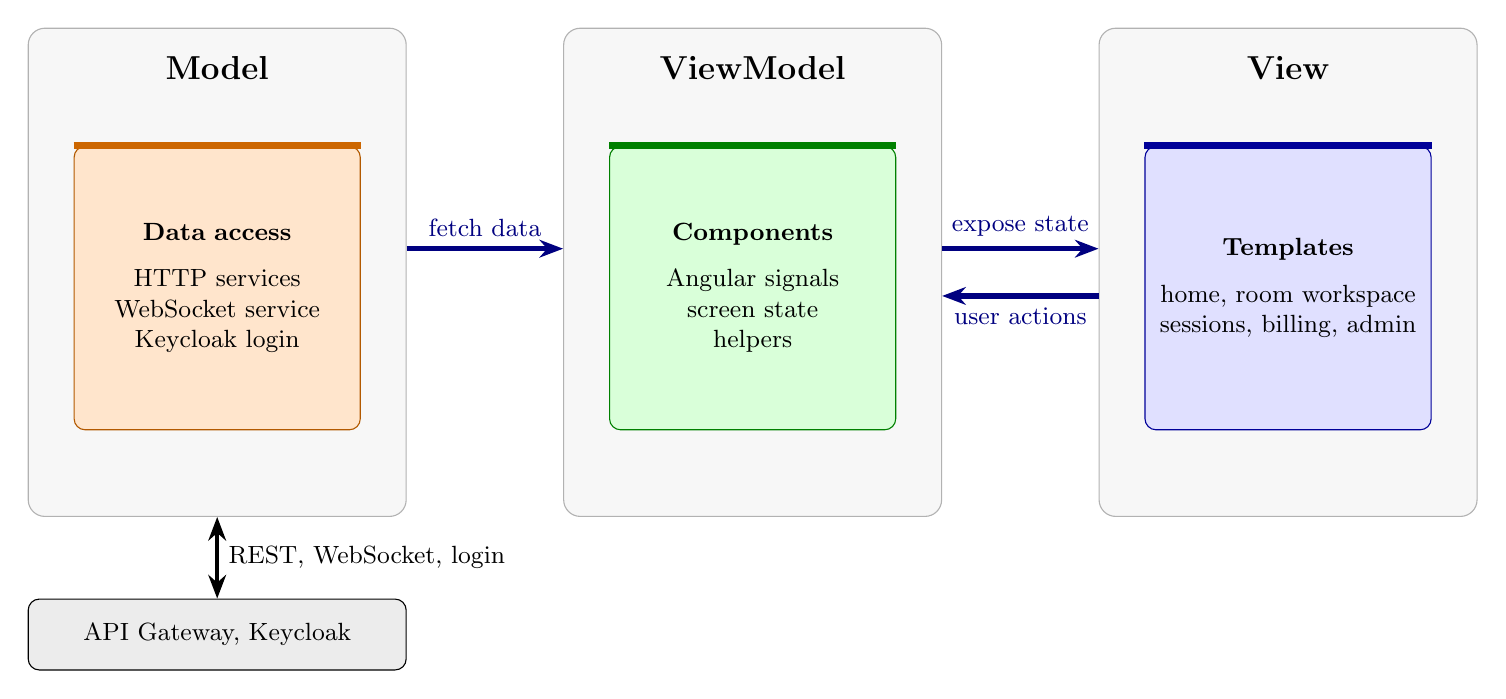
\begin{tikzpicture}[
  panel/.style={draw=gray!60, rounded corners=6pt, fill=gray!6, minimum width=4.8cm, minimum height=6.2cm},
  inner/.style={draw, rounded corners=4pt, align=center, text width=3.4cm, minimum height=3.6cm, font=\small},
  title/.style={font=\large\bfseries}]
  % panels
  \node[panel] (pm) at (0,0) {};
  \node[panel] (pv) at (6.8,0) {};
  \node[panel] (pw) at (13.6,0) {};
  \node[title] at (0,2.6) {Model};
  \node[title] at (6.8,2.6) {ViewModel};
  \node[title] at (13.6,2.6) {View};
  % inner boxes
  \node[inner, fill=orange!20, draw=orange!70!black] (m) at (0,-0.2) {\textbf{Data access}\\[2mm]HTTP services\\WebSocket service\\Keycloak login};
  \node[inner, fill=green!15, draw=green!50!black] (vm) at (6.8,-0.2) {\textbf{Components}\\[2mm]Angular signals\\screen state\\helpers};
  \node[inner, fill=blue!12, draw=blue!60!black] (v) at (13.6,-0.2) {\textbf{Templates}\\[2mm]home, room workspace\\sessions, billing, admin};
  \draw[line width=2.5pt, orange!80!black] (m.north west) -- (m.north east);
  \draw[line width=2.5pt, green!50!black] (vm.north west) -- (vm.north east);
  \draw[line width=2.5pt, blue!60!black] (v.north west) -- (v.north east);
  % arrows
  \draw[-{Stealth[length=3mm]}, line width=2pt, blue!50!black] ([yshift=0.3cm]pm.east) -- node[above, font=\small]{fetch data} ([yshift=0.3cm]pv.west);
  \draw[-{Stealth[length=3mm]}, line width=2pt, blue!50!black] ([yshift=0.3cm]pv.east) -- node[above, font=\small]{expose state} ([yshift=0.3cm]pw.west);
  \draw[-{Stealth[length=3mm]}, line width=2pt, blue!50!black] ([yshift=-0.3cm]pw.west) -- node[below, font=\small]{user actions} ([yshift=-0.3cm]pv.east);
  % backend
  \node[draw, rounded corners=4pt, fill=gray!15, minimum width=4.8cm, minimum height=0.9cm, font=\small] (gw) at (0,-4.6) {API Gateway, Keycloak};
  \draw[{Stealth[length=3mm]}-{Stealth[length=3mm]}, line width=1.5pt] (pm.south) -- node[right, font=\small]{REST, WebSocket, login} (gw.north);
\end{tikzpicture}}
\caption{Frontend architecture of MindSpark (MVVM with Angular)}
\label{fig:arch-frontend}
\end{figure}

\begin{itemize}
  \item \textbf{Model:} the data layer. One HTTP service per business area, a WebSocket service for the room, and the Keycloak login. An interceptor adds the token to every request, and guards protect private and admin pages.
  \item \textbf{ViewModel:} the page and component classes. They keep the screen state in Angular signals, such as ideas, online users and cursors, with small helpers for card and drawing positions.
  \item \textbf{View:} the templates. They only display the state and send user actions.
\end{itemize}

% ---------------------------------------------------------------------
\subsection{Backend Architecture}
\label{subsec:arch-backend}

The core backend is a layered Spring Boot application. Figure~\ref{fig:arch-backend} shows how a request flows through it, and Figure~\ref{fig:arch-ai} shows the AI service, which is built as a separate pipeline.

\begin{figure}[htbp]
\centering
\hyphenpenalty=10000\relax
\fitwidth{%
\begin{tikzpicture}
  \node[grey, text width=4cm] (req) at (0,11) {HTTP or WebSocket request};
  \node[blue, text width=4.4cm] (sec) at (0,9.4) {\textbf{Security}\\JWT check, roles};
  \node[green, text width=4.4cm] (ctl) at (0,7.8) {\textbf{Controllers}\\REST endpoints};
  \node[grey, text width=3cm] (dto) at (6.0,7.8) {\textbf{DTOs}\\requests, responses};
  \node[blue, text width=4.4cm, minimum height=1.4cm] (srv) at (0,5.8) {\textbf{Services}\\rooms, ideas, votes, comments, vote pools, drawings, presence, session export};
  \node[green, text width=4.4cm] (rep) at (0,3.7) {\textbf{Repositories}\\Spring Data JPA};
  \node[orange, text width=4.4cm] (ent) at (0,2.1) {\textbf{Entities}\\JPA models};
  \node[grey, text width=4.4cm] (db) at (0,0.5) {\textbf{PostgreSQL}};
  \draw[flow] (req) -- (sec);
  \draw[flow] (sec) -- (ctl);
  \draw[flow, <->] (ctl) -- node[lab]{validates} (dto);
  \draw[flow] (ctl) -- node[lab,right]{calls} (srv);
  \draw[flow] (srv) -- node[lab,right]{calls} (rep);
  \draw[flow] (rep) -- node[lab,right]{maps} (ent);
  \draw[flow] (ent) -- node[lab,right]{SQL} (db);
  % left side: quota guard and kafka
  \node[orange, text width=3.2cm] (qg) at (-6.2,7.6) {\textbf{Quota guard}\\entitlement client};
  \node[orange, text width=3.2cm] (subs) at (-6.2,9.6) {\textbf{Subscription Service}};
  \node[grey, text width=3.2cm] (kp) at (-6.2,4.2) {\textbf{Event producer}};
  \node[orange, text width=3.2cm] (kf) at (-6.2,2.6) {\textbf{Kafka}};
  \draw[flow] (srv.west) -| (qg.south);
  \draw[flow] (qg) -- node[lab,right]{plan limits} (subs);
  \draw[flow] (srv.west) -| (kp.north);
  \draw[flow] (kp) -- (kf);
  % right side: websocket
  \node[blue, text width=3.2cm] (ev) at (6.2,4.2) {\textbf{Event listener}\\after commit};
  \node[blue, text width=3.2cm] (ws) at (6.2,2.6) {\textbf{WebSocket handler}\\room channels};
  \node[green, text width=3.2cm] (cl) at (6.2,1.0) {\textbf{Web clients}};
  \draw[flow] (srv.east) -| (ev.north);
  \draw[flow] (ev) -- (ws);
  \draw[flow] (ws) -- node[lab,right]{broadcast} (cl);
\end{tikzpicture}}
\caption{Core backend architecture of MindSpark}
\label{fig:arch-backend}
\end{figure}

\begin{itemize}
  \item \textbf{Security:} validates the JWT and turns the realm roles into permissions before any controller runs.
  \item \textbf{Controllers:} expose the REST endpoints and validate input with DTOs. They mostly delegate to services. A few simple lookups, such as reading the current user, use a repository directly.
  \item \textbf{Services:} hold the business rules, grouped by feature (room, idea, vote, comment, drawing, and so on). They are the main layer that talks to the repositories and to the other components below.
  \item \textbf{Repositories and entities:} Spring Data JPA maps the entities to PostgreSQL. Code is organised by feature, so each feature keeps its entity, repository and service together.
  \item \textbf{Quota guard:} asks the subscription service for the user's plan limits before creating a room or adding a participant. A circuit breaker protects this call.
  \item \textbf{Real-time delivery:} after a database commit, an event listener asks the WebSocket handler to broadcast the change to the room. Nothing is sent if the transaction fails.
  \item \textbf{Event producer:} publishes room-closed and vote-pool-closed events to Kafka for the notification service.
  \item \textbf{Internal endpoints:} a few endpoints under \texttt{/internal} give room data to the session service and room access checks to the media service. They need a shared service key and are not exposed through the gateway.
\end{itemize}

\begin{figure}[htbp]
\centering
\hyphenpenalty=10000\relax
\fitwidth{%
\begin{tikzpicture}
  \node[green, text width=2.9cm] (ctl) at (0,4) {\textbf{AI Controller}\\JWT, REST};
  \node[blue, text width=3.6cm, minimum height=1.5cm] (orc) at (4.8,4) {\textbf{Orchestrator}\\one flow per tool, payload cap, limit on simultaneous calls};
  \node[grey, text width=2.9cm] (pb) at (0,6.4) {\textbf{Prompt builders}\\topic and ideas as context};
  \node[blue, text width=2.9cm] (qg) at (4.8,6.6) {\textbf{Quota guard}\\daily limit per tier};
  \node[grey, text width=2.9cm] (usage) at (9.4,6.6) {\textbf{Usage database}};
  \node[grey, text width=2.9cm] (val) at (9.4,4) {\textbf{Output validation}\\JSON structure};
  \node[blue, text width=2.9cm] (rt) at (4.8,1.4) {\textbf{Model router}\\fallback order};
  \node[blue, text width=2.9cm] (cli) at (9.4,1.4) {\textbf{LLM client}\\OpenAI-compatible};
  \node[orange, text width=2.9cm] (prov) at (14,1.4) {\textbf{Gemini, Groq}};
  \draw[flow] (ctl) -- (orc);
  \draw[flow] (pb) -- (orc);
  \draw[flow, <->] (orc) -- (qg);
  \draw[flow, <->] (qg) -- (usage);
  \draw[flow, <->] (orc) -- (val);
  \draw[flow] (orc) -- (rt);
  \draw[flow] (rt) -- (cli);
  \draw[flow] (cli) -- (prov);
\end{tikzpicture}}
\caption{AI service pipeline}
\label{fig:arch-ai}
\end{figure}

\begin{itemize}
  \item \textbf{Orchestrator and prompt builders:} each AI tool has its own prompt, built from the room topic and the ideas involved. The orchestrator rejects oversized requests, limits how many calls run at the same time, and gives the quota back if the call fails.
  \item \textbf{Quota guard:} counts each user's AI calls per day in its own database and applies the limit of their tier before any model is called. The tier is read from the token: a user with the \texttt{premium} role gets the premium models and a higher limit, anyone else gets the free tier.
  \item \textbf{Output validation:} the model must answer in a fixed JSON structure. A malformed answer is rejected rather than shown.
  \item \textbf{Model router and LLM client:} the router tries the models configured for the tier in order (Gemini for the free tier, Groq for the premium tier) and falls back to the next one when a model fails or is rate limited. A circuit breaker stops calls when the providers keep failing.
\end{itemize}

% ---------------------------------------------------------------------
\subsection{Justification of Architectural Choices}
\label{subsec:arch-justif}

\begin{itemize}
  \item \textbf{Separation of concerns:} each service owns one business area and its data, and each layer inside a service has one job.
  \item \textbf{Scalability:} services are deployed and scaled independently. The AI service, for example, can be limited without affecting rooms.
  \item \textbf{Security:} Keycloak centralises identity, and every backend service validates tokens itself, so no service trusts the network.
  \item \textbf{Resilience:} circuit breakers, provider fallback and per-plan quotas keep one failure from stopping the platform.
  \item \textbf{Testability:} services, controllers and the frontend data layer can be tested separately.
\end{itemize}


% =====================================================================
% Chapter 3 -- Part 2: Section 3.7 (Scrum Approach and Product Backlog)
% Author: Ilyes
%
% Extra packages needed in the main preamble:
%   \usepackage{longtable}
%   \usepackage{booktabs}
%   \usepackage{tikz}
%   \usetikzlibrary{arrows.meta}
%
% Paste after sections 3.5 and 3.6 (section numbers are automatic).
% =====================================================================

\section{Scrum Approach and Product Backlog}
\label{sec:scrum}

The project follows the Scrum framework introduced in Chapter~1. This section presents the team, the user stories, the product backlog and the release plan.

% ---------------------------------------------------------------------
\subsection{Scrum Team Composition}
\label{subsec:scrum-team}

The team has six members and no Scrum Master. Khoula Jridi is the Product Owner and sets the priorities. The six students form the Development Team, and each one owns a part of the platform and a chapter of this report.

\begin{figure}[htbp]
\centering
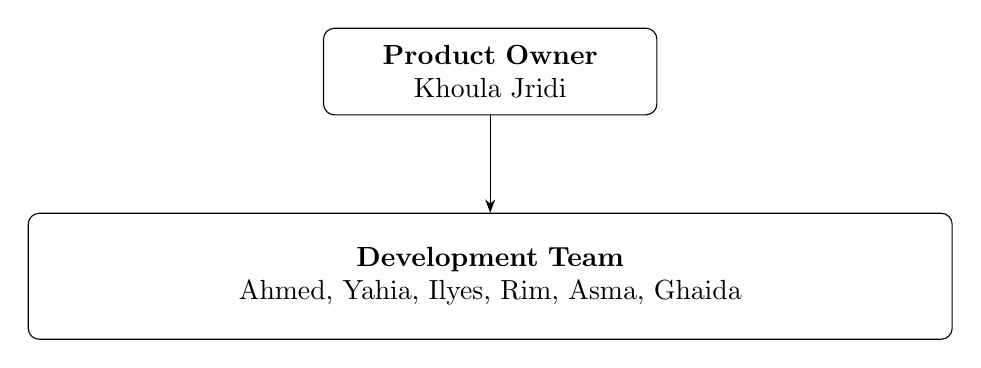
\begin{tikzpicture}[box/.style={draw, rounded corners, align=center, minimum height=1.1cm, text width=4cm}]
\node[box] (po) at (0,0) {\textbf{Product Owner}\\Khoula Jridi};
\node[draw, rounded corners, align=center, text width=11.5cm, minimum height=1.6cm] (dev) at (0,-2.6) {\textbf{Development Team}\\Ahmed, Yahia, Ilyes, Rim, Asma, Ghaida};
\draw[-{Stealth}] (po) -- (dev);
\end{tikzpicture}
\caption{Scrum team composition}
\label{fig:scrum-team}
\end{figure}

% ---------------------------------------------------------------------
\subsection{User Stories and Technical Enablers}
\label{subsec:user-stories}

The user stories are grouped by actor. Participant stories are written by a visitor, a user or a client (see Table~\ref{tab:role-mapping}). The technical stories are enablers for the team: they have no end user but make the other stories possible.

\subsubsection*{Participant}

\begin{longtable}{@{}p{0.10\textwidth}p{0.75\textwidth}@{}}
\toprule
\textbf{ID} & \textbf{User story} \\
\midrule
\endfirsthead
\toprule
\textbf{ID} & \textbf{User story} \\
\midrule
\endhead
\bottomrule
\endfoot
US-1 & As a visitor, I can register with my name, email and password. \\
US-2 & As a user, I can log in with my email and password. \\
US-3 & As a user, I can log out. \\
US-4 & As a client, I can view my profile. \\
US-5 & As a client, I can edit my name and avatar. \\
US-6 & As a user, I can reset a forgotten password by email. \\
US-7 & As a client, I can change my password. \\
US-8 & As a client, I can delete my account. \\
US-9 & As a client, I can create a brainstorming room. \\
US-10 & As a client, I can join a room using an invitation code. \\
US-11 & As a client, I can leave a brainstorming room. \\
US-12 & As a client, I can see all rooms I created and reopen them later. \\
US-22 & As a client, I can create an idea in a room I belong to. \\
US-23 & As a client, I can edit my own ideas. \\
US-24 & As a client, I can delete my own ideas. \\
US-25 & As a client, I can view all participants' ideas in my room. \\
US-26 & As a client, I can attach images to my idea. \\
US-27 & As a client, I can organise ideas into categories. \\
US-28 & As a client, I can create, rename and delete categories in a room. \\
US-29 & As a client, I can search ideas by keyword. \\
US-30 & As a client, I can filter ideas by category, author and minimum votes, and sort them. \\
US-32 & As a client, I can comment on an idea. \\
US-33 & As a client, I can edit or delete my own comments. \\
US-34 & As a client, I can reply to a comment. \\
US-35 & As a client, I can vote for an idea. \\
US-36 & As a client, I can remove or change my vote. \\
US-39 & As a client, I can see new ideas, comments and votes live. \\
US-40 & As a client, I can see who is currently online in the room. \\
US-41 & As a client, I can see other participants' cursors live. \\
US-43 & As a client, I can use AI to generate ideas based on a topic. \\
US-44 & As a client, I can use AI to improve or expand an idea. \\
US-45 & As a client, I can use AI to group similar ideas. \\
US-46 & As a client, I can use AI to summarise a brainstorming session. \\
US-47 & As a client, I can use AI to find risks in a selected idea. \\
US-48 & As a client, I can use AI to compare 2 to 4 selected ideas. \\
US-49 & As a client, I can convert selected ideas into an action plan. \\
US-52 & As a client, I can save and revisit my brainstorming sessions. \\
US-53 & As a client, I can export the results of a session. \\
US-54 & As a client, I can view the available plans. \\
US-55 & As a client, I can subscribe to a plan. \\
US-56 & As a client, I can upgrade or downgrade my plan. \\
US-57 & As a client, I can cancel my subscription. \\
US-58 & As a client, I can view my billing history. \\
US-59 & As a client, I can use the platform within the limits of my plan (rooms, participants, AI calls). \\
\end{longtable}

\subsubsection*{Room Creator}

\begin{longtable}{@{}p{0.10\textwidth}p{0.75\textwidth}@{}}
\toprule
\textbf{ID} & \textbf{User story} \\
\midrule
\endfirsthead
\toprule
\textbf{ID} & \textbf{User story} \\
\midrule
\endhead
\bottomrule
\endfoot
US-13 & As a room creator, I can edit the room details. \\
US-14 & As a room creator, I can preview the participants list. \\
US-15 & As a room creator, I can remove a participant. \\
US-16 & As a room creator, I can close the room. \\
US-17 & As a room creator, I can delete the room. \\
US-37 & As a room creator, I can create a vote pool. \\
\end{longtable}

\subsubsection*{Technical enablers}

T1 to T7 are team stories. US-38 and US-42 are written from the developer's point of view.

\begin{longtable}{@{}p{0.10\textwidth}p{0.75\textwidth}@{}}
\toprule
\textbf{ID} & \textbf{User story} \\
\midrule
\endfirsthead
\toprule
\textbf{ID} & \textbf{User story} \\
\midrule
\endhead
\bottomrule
\endfoot
T1 & As a team, we can work in a shared repository with branching rules and an automated build. \\
T2 & As a team, we can run a frontend, backend and database connected end-to-end. \\
T3 & As a team, we can create the first schema and migrations. \\
T4 & As a team, we can access a public demo environment. \\
T5 & As a team, we can reset the demo to a known state. \\
T6 & As a team, we can run automated tests for the critical flows. \\
T7 & As a team, we can harden the platform before real users. \\
US-38 & As a developer, I can use an authenticated real-time channel per room (enabler). \\
US-42 & As a developer, I can use a backend AI service wrapping the LLM provider (enabler). \\
\end{longtable}

% ---------------------------------------------------------------------
\subsection{Prioritized Product Backlog}
\label{subsec:backlog}

The product backlog holds \textbf{52 user stories} and \textbf{7 technical enablers}, \textbf{59 items} in all. Story numbers follow the original user-story document, which is why some are skipped. Priorities use the MoSCoW scale: \textit{Must} is needed for the demo and the product, \textit{Should} is important, and \textit{Could} is dropped first if time runs short. The backlog has 29 Must, 24 Should and 6 Could items, spread over the three sprints as $18+21+20=59$.

\begin{longtable}{@{}p{0.09\textwidth}p{0.17\textwidth}p{0.40\textwidth}p{0.11\textwidth}p{0.09\textwidth}@{}}
\toprule
\textbf{ID} & \textbf{Theme} & \textbf{User story} & \textbf{Priority} & \textbf{Sprint} \\
\midrule
\endfirsthead
\toprule
\textbf{ID} & \textbf{Theme} & \textbf{User story} & \textbf{Priority} & \textbf{Sprint} \\
\midrule
\endhead
\bottomrule
\endfoot
T1 & Foundation & We can work in a shared repository with branching rules and an automated build. & Must & 1 \\
T2 & Foundation & We can run a frontend, backend and database connected end-to-end. & Must & 1 \\
T3 & Foundation & We can create the first schema and migrations. & Must & 1 \\
T4 & Foundation & We can access a public demo environment. & Must & 1 \\
US-1 & Authentication & I can register with my name, email and password. & Must & 1 \\
US-2 & Authentication & I can log in with my email and password. & Must & 1 \\
US-3 & Authentication & I can log out. & Must & 1 \\
US-4 & Authentication & I can view my profile. & Must & 1 \\
US-9 & Rooms & I can create a brainstorming room. & Must & 1 \\
US-10 & Rooms & I can join a room using an invitation code. & Must & 1 \\
US-11 & Rooms & I can leave a brainstorming room. & Must & 1 \\
US-12 & Rooms & I can see all rooms I created and reopen them later. & Must & 1 \\
US-22 & Ideas and votes & I can create an idea in a room I belong to. & Must & 1 \\
US-23 & Ideas and votes & I can edit my own ideas. & Must & 1 \\
US-24 & Ideas and votes & I can delete my own ideas. & Must & 1 \\
US-25 & Ideas and votes & I can view all participants' ideas in my room. & Must & 1 \\
US-35 & Ideas and votes & I can vote for an idea. & Must & 1 \\
US-36 & Ideas and votes & I can remove or change my vote. & Must & 1 \\
US-38 & Real-time & I can use an authenticated real-time channel per room (enabler). & Must & 2 \\
US-39 & Real-time & I can see new ideas, comments and votes live. & Must & 2 \\
US-40 & Real-time & I can see who is currently online in the room. & Must & 2 \\
US-41 & Real-time & I can see other participants' cursors live. & Must & 2 \\
US-32 & Comments & I can comment on an idea. & Must & 2 \\
US-33 & Comments & I can edit or delete my own comments. & Should & 2 \\
US-34 & Comments & I can reply to a comment. & Should & 2 \\
US-27 & Idea organisation & I can organise ideas into categories. & Should & 2 \\
US-28 & Idea organisation & I can create, rename and delete categories in a room. & Should & 2 \\
US-29 & Idea organisation & I can search ideas by keyword. & Should & 2 \\
US-30 & Idea organisation & I can filter ideas by category, author and minimum votes, and sort them. & Should & 2 \\
US-13 & Room management & I can edit the room details. & Should & 2 \\
US-14 & Room management & I can preview the participants list. & Should & 2 \\
US-15 & Room management & I can remove a participant. & Should & 2 \\
US-16 & Room management & I can close the room. & Should & 2 \\
US-17 & Room management & I can delete the room. & Could & 2 \\
US-42 & AI core and profile & I can use a backend AI service wrapping the LLM provider (enabler). & Must & 2 \\
US-43 & AI core and profile & I can use AI to generate ideas based on a topic. & Must & 2 \\
US-44 & AI core and profile & I can use AI to improve or expand an idea. & Must & 2 \\
US-5 & AI core and profile & I can edit my name and avatar. & Should & 2 \\
T5 & AI core and profile & We can reset the demo to a known state. & Should & 2 \\
US-54 & Subscriptions & I can view the available plans. & Must & 3 \\
US-55 & Subscriptions & I can subscribe to a plan. & Must & 3 \\
US-59 & Subscriptions & I can use the platform within the limits of my plan (rooms, participants, AI calls). & Must & 3 \\
US-56 & Subscriptions & I can upgrade or downgrade my plan. & Should & 3 \\
US-57 & Subscriptions & I can cancel my subscription. & Should & 3 \\
US-58 & Subscriptions & I can view my billing history. & Should & 3 \\
US-45 & Advanced AI & I can use AI to group similar ideas. & Should & 3 \\
US-46 & Advanced AI & I can use AI to summarise a brainstorming session. & Should & 3 \\
US-49 & Advanced AI & I can convert selected ideas into an action plan. & Should & 3 \\
US-47 & Advanced AI & I can use AI to find risks in a selected idea. & Could & 3 \\
US-48 & Advanced AI & I can use AI to compare 2 to 4 selected ideas. & Could & 3 \\
US-52 & History, votes and media & I can save and revisit my brainstorming sessions. & Should & 3 \\
US-53 & History, votes and media & I can export the results of a session. & Should & 3 \\
US-37 & History, votes and media & I can create a vote pool. & Could & 3 \\
US-26 & History, votes and media & I can attach images to my idea. & Could & 3 \\
US-6 & Account & I can reset a forgotten password by email. & Should & 3 \\
US-7 & Account & I can change my password. & Should & 3 \\
US-8 & Account & I can delete my account. & Could & 3 \\
T6 & Quality & We can run automated tests for the critical flows. & Should & 3 \\
T7 & Quality & We can harden the platform before real users. & Should & 3 \\
\end{longtable}

% ---------------------------------------------------------------------
\subsection{Three-Sprint Release Roadmap}
\label{subsec:roadmap}

The work is split into three sprints. Each one ends with something that can be shown, and the first one already gives a working demo on a public URL.

\begin{figure}[htbp]
\centering
\hyphenpenalty=10000
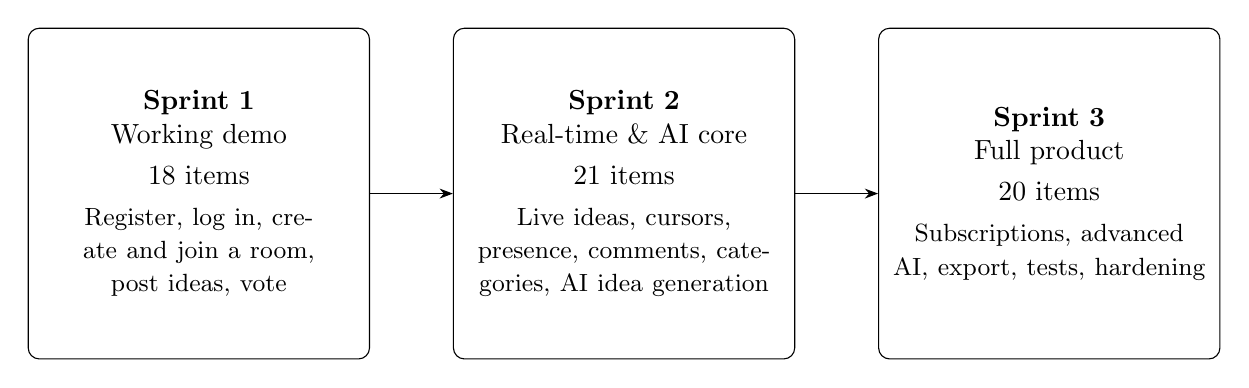
\begin{tikzpicture}[box/.style={draw, rounded corners, align=center, text width=4.1cm, minimum height=4.2cm}]
\node[box] (s1) at (0,0) {\textbf{Sprint 1}\\Working demo\\[1mm]18 items\\[1mm]\small Register, log in, create and join a room, post ideas, vote};
\node[box] (s2) at (5.4,0) {\textbf{Sprint 2}\\Real-time \& AI core\\[1mm]21 items\\[1mm]\small Live ideas, cursors, presence, comments, categories, AI idea generation};
\node[box] (s3) at (10.8,0) {\textbf{Sprint 3}\\Full product\\[1mm]20 items\\[1mm]\small Subscriptions, advanced AI, export, tests, hardening};
\draw[-{Stealth}] (s1) -- (s2);
\draw[-{Stealth}] (s2) -- (s3);
\end{tikzpicture}
\caption{Three-sprint release roadmap}
\label{fig:roadmap}
\end{figure}

% =====================================================================
% Chapter 3 -- Part 5: Section 3.8 (Conclusion)
% Author: Ilyes
% =====================================================================

\section{Conclusion}
\label{sec:req-conclusion}

This chapter defined what MindSpark must do and how it is built. We identified four actors, grouped the 52 user stories into six families of functional requirements, and set ten quality requirements. The use case diagrams present the system theme by theme, and the architecture shows an Angular web app and a set of services behind one gateway. The Scrum backlog holds 59 items spread over three sprints of 18, 21 and 20 items. The next three chapters follow these sprints one by one.

\end{document}